\def \tikzexa
{
\begin{tikzpicture}[
	scale=0.75,
	start chain=1 going below, 
	start chain=2 going right,
	node distance=1mm,
	desc/.style={
		scale=0.75,
		on chain=2,
		rectangle,
		rounded corners,
		draw=black, 
		very thick,
		text centered,
		text width=8cm,
		minimum height=12mm,
		fill=blue!30
		},
	it/.style={
		fill=blue!10
	},
	level/.style={
		scale=0.75,
		on chain=1,
		minimum height=12mm,
		text width=2cm,
		text centered
	},
	every node/.style={font=\sffamily}
]

% Levels
\node [level] (Level 5) {Level 5};
\node [level] (Level 4) {Level 4};
\node [level] (Level 3) {Level 3};
\node [level] (Level 2) {Level 2};
\node [level] (Level 1.5) { };
\node [level] (Level 1) {Level 1};
\node [level] (Level 0) {Level 0};

% Descriptions
\chainin (Level 5); % Start right of Level 5
% IT levels
\node [desc, it] (Archives) {Archives/File Servers};
\node [desc, it, continue chain=going below] (ERP) {ERP/Finance/Messaging};
% ICS levels
\node [desc] (Operations) {Operations Management/Historians};
\node [desc] (Supervisory) {Supervisory Controls};
\node [desc, text width=3.5cm, xshift=2.25cm] (PLC) {PLC/RTU IP Communication};
\node [desc, text width=3.5cm, xshift=-4.5cm] (SIS) {Safety Instrumented Systems};
\node [desc, xshift=2.25cm] (IO) {I/O from Sensors};
\end{tikzpicture}
}






\def \tikzexb
{
\begin{tikzpicture}
\draw[gray,fill=gray,path fading=south] (0,0) rectangle +(0.3,-0.3);% <- MAGIC
  % (if this is not present none of the shadings work)

%top
\shade[left color=black!10!white,right color=black!40!white] (-1,0.75)
  -- ++(2,0) -- ++(0.25,-0.25) -- ++(-2.5,0) -- cycle;
\draw (-1,0.75) -- ++(2,0) -- ++(0.25,-0.25) -- ++(-2.5,0) -- cycle;

%source
\shade[left color=black!10!white,right color=black!40!white] (1.25,0.5)
  -- ++(0,-1.75) -- ++(-2.5,0) -- ++(0,1.75) -- cycle;
\draw (1.25,0.5) -- ++(0,-1.75) -- ++(-2.5,0) -- ++(0,1.75) -- cycle;

%top condenser system
\shade[left color=black!10!white,right color=black!40!white] (1.25,-1.25)
  -- ++(0.25,-0.25) -- ++(-3,0) -- ++(0.25,0.25) -- cycle;
\draw (1.25,-1.25) -- ++(0.25,-0.25) -- ++(-3,0) -- ++(0.25,0.25) -- cycle;

%condenser system
\shade[left color=black!10!white,right color=black!40!white] (1.5,-1.5)
  -- ++(0,-2) -- ++(-3,0) -- ++(0,2) -- cycle;
\draw (1.5,-1.5) -- ++(0,-2) -- ++(-3,0) -- ++(0,2) -- cycle;

%condenser bottom
\shade[left color=black!10!white,right color=black!40!white] (1.5,-3.5)
  -- ++(-0.25,-0.25) -- ++(-2.5,0) -- ++(-0.25,0.25) -- cycle;
\draw (1.5,-3.5) -- ++(-0.25,-0.25) -- ++(-2.5,0) -- ++(-0.25,0.25) -- cycle;

%specimen and objective
\shade[left color=black!10!white,right color=black!40!white] (1.25,-3.75)
  -- ++(0,-2.5) -- ++(-2.5,0) -- ++(0,2.5) -- cycle;
\draw (1.25,-3.75) -- ++(0,-2.5) -- ++(-2.5,0) -- ++(0,2.5) -- cycle;

%projector system top
\shade[left color=black!10!white,right color=black!40!white] (1.25,-6.25)
  -- ++(0.25,-0.25) -- ++(-3,0) -- ++(0.25,0.25) -- cycle;
\draw (1.25,-6.25) -- ++(0.25,-0.25) -- ++(-3,0) -- ++(0.25,0.25) -- cycle;

%projector system
\shade[left color=black!10!white,right color=black!40!white] (1.5,-6.5)
  -- ++(0,-1.5) -- ++(-3,0) -- ++(0,1.5) -- cycle;
\draw (1.5,-6.5) -- ++(0,-1.5) -- ++(-3,0) -- ++(0,1.5) -- cycle;

%image
\shade[left color=black!10!white,right color=black!40!white] (1.5,-8)
  -- ++(1,-1.5) -- ++(0,-0.75) -- ++(-5,0) -- ++(0,0.75) -- ++(1,1.5) -- cycle;
\draw (1.5,-8) -- ++(1,-1.5) -- ++(0,-0.75) -- ++(-5,0) -- ++(0,0.75)
  -- ++(1,1.5) -- cycle;

%sample entrance
\shade[left color=black!10!white,right color=black!40!white] (-1.25,-4.5)
  -- ++(-0.5,0) -- ++(-0.2,-0.2) -- ++(0,-0.6) -- ++(0.2,-0.2)
  -- ++(0.5,0) -- cycle;
\draw (-1.25,-4.5) -- ++(-0.5,0) -- ++(-0.2,-0.2) -- ++(0,-0.6)
  -- ++(0.2,-0.2)  -- ++(0.5,0) -- cycle;

%sample holder
\draw[fill=black] (-1.95,-4.8) -- ++(-0.08,0) -- ++(-0.02,-0.02)
  -- ++(0,-0.36) -- ++(0.02,-0.02) -- ++(0.08,0) -- cycle;

%inside
\begin{scope}
  \path[clip,decoration={random steps, segment length=6pt, amplitude=2pt},
	  decorate] (0,0.5) -- ++(0.4,0) -- ++(0.4,-0.4) -- ++(0,-8.5)
	  -- ++(1,-1.3) -- ++(-0.4,-0.4) -- ++(-2.8,0) -- ++(-0.4,0.4)
	  -- ++(1,1.3) -- ++(0,8.5) -- ++(0.4,0.4) -- cycle;
  \shade[left color=black!40!white,right color=black!10!white] (-1,0.75)
	  -- ++(2,0) -- ++(0.25,-0.25) -- ++(0,-1.75) -- ++(0.25,-0.25) -- ++(0,-2)
	  -- ++(-0.25,-0.25) -- ++(0,-2.5) -- ++(0.25,-0.25) -- ++(0,-1.5)
	  -- ++(1,-1.5) -- ++(0,-0.75) -- ++(-5,0) -- ++(0,0.75) -- ++(1,1.5)
	  -- ++ (0,1.5) -- ++(0.25,0.25) -- ++(0,2.5) -- ++(-0.25,0.25) -- ++(0,2)
	  -- ++(0.25,0.25) -- ++(0,1.75) -- cycle;

%source
\draw (-0.25,0.15) -- ++(0,-0.05) .. controls +(0,-0.08) and +(-0.08,0)
  .. ++(0.1,-0.1) -- ++(0.05,0) .. controls +(0.08,0) and +(0,0.08)
  .. ++(0.1,-0.1) .. controls +(0,0.08) and +(-0.08,0) .. ++(0.1,0.1) --
  ++(0.05,0) .. controls +(0.08,0) and +(0,-0.08) .. ++(0.1,0.1) -- ++(0,0.05);

%C1
\draw[fill=brown!80!yellow] (-0.4,-1.75) -- ++(-0.5,0) -- ++(0,-0.5)
  -- ++(0.5,0) -- cycle;
\draw (-0.4,-1.75) ++(-0.04,-0.04) -- ++(-0.42,0) -- ++(0,-0.42)
  -- ++(0.42,0) -- cycle;
\begin{scope}
  \path[clip,draw] (-0.4,-1.75) ++(-0.04,-0.04) -- ++(-0.42,0)
	  -- ++(0,-0.42) -- ++(0.42,0) -- cycle;
  \foreach \j in {-0.07,-0.14,...,-0.42}
	  \foreach \i in {-0.07,-0.14,...,-0.42} {
		  \draw[fill=brown!40!yellow] (-0.4,-1.75) ++(-0.04,-0.04)
			  ++(0.035,0.035) ++(\i,\j) circle (0.035);
	  }
\end{scope}
\draw[fill=brown!80!yellow] (0.9,-1.75) -- ++(-0.5,0) -- ++(0,-0.5)
  -- ++(0.5,0) -- cycle;
\draw (0.9,-1.75) ++(-0.04,-0.04) -- ++(-0.42,0) -- ++(0,-0.42)
  -- ++(0.42,0) -- cycle;
\begin{scope}
  \path[clip,draw] (0.9,-1.75) ++(-0.04,-0.04) -- ++(-0.42,0)
	  -- ++(0,-0.42) -- ++(0.42,0) -- cycle;
  \foreach \j in {-0.07,-0.14,...,-0.42}
	  \foreach \i in {-0.07,-0.14,...,-0.42} {
		  \draw[fill=brown!40!yellow] (0.9,-1.75) ++(-0.04,-0.04)
			  ++(0.035,0.035) ++(\i,\j) circle (0.035);
	  }
\end{scope}

%C2
\draw[fill=brown!80!yellow] (-0.4,-2.75) -- ++(-0.5,0) -- ++(0,-0.5)
  -- ++(0.5,0) -- cycle;
\draw (-0.4,-2.75) ++(-0.04,-0.04) -- ++(-0.42,0) -- ++(0,-0.42)
  -- ++(0.42,0) -- cycle;
\begin{scope}
  \path[clip,draw] (-0.4,-2.75) ++(-0.04,-0.04) -- ++(-0.42,0)
	  -- ++(0,-0.42) -- ++(0.42,0) -- cycle;
  \foreach \j in {-0.07,-0.14,...,-0.42}
	  \foreach \i in {-0.07,-0.14,...,-0.42} {
		  \draw[fill=brown!40!yellow] (-0.4,-2.75) ++(-0.04,-0.04)
			  ++(0.035,0.035) ++(\i,\j) circle (0.035);
	  }
\end{scope}
\draw[fill=brown!80!yellow] (0.9,-2.75) -- ++(-0.5,0) -- ++(0,-0.5)
  -- ++(0.5,0) -- cycle;
\draw (0.9,-2.75) ++(-0.04,-0.04) -- ++(-0.42,0) -- ++(0,-0.42)
  -- ++(0.42,0) -- cycle;
\begin{scope}
  \path[clip,draw] (0.9,-2.75) ++(-0.04,-0.04) -- ++(-0.42,0)
	  -- ++(0,-0.42) -- ++(0.42,0) -- cycle;
  \foreach \j in {-0.07,-0.14,...,-0.42}
	  \foreach \i in {-0.07,-0.14,...,-0.42} {
		  \draw[fill=brown!40!yellow] (0.9,-2.75) ++(-0.04,-0.04)
			  ++(0.035,0.035) ++(\i,\j) circle (0.035);
	  }
\end{scope}

%condenser aperture
\draw[fill=black] (-1,-3.45) -- ++(0.6,0) -- ++(-0.1,-0.1)
  -- ++(-0.5,0) -- cycle;
\draw[fill=black] (1,-3.45) -- ++(-0.6,0) -- ++(0.1,-0.1)
  -- ++(0.5,0) -- cycle;

%specimen
\draw[fill=brown!70!yellow] (-1,-4.95) -- ++(0.75,0) -- ++(0.05,-0.045)
  -- ++(0,-0.01) -- ++(-0.05,-0.045) -- ++(-0.75,0) -- cycle;
\draw[fill=black] (-0.2,-4.995) -- ++(0.4,0) -- ++(0,-0.01)
  -- ++(-0.4,0) -- cycle;
  
%objective
\draw[fill=brown!80!yellow] (-0.4,-5.25) -- ++(-0.5,0) -- ++(0,-0.5)
  -- ++(0.5,0) -- cycle;
\draw (-0.4,-5.25) ++(-0.04,-0.04) -- ++(-0.42,0) -- ++(0,-0.42)
  -- ++(0.42,0) -- cycle;
\begin{scope}
  \path[clip,draw] (-0.4,-5.25) ++(-0.04,-0.04) -- ++(-0.42,0)
	  -- ++(0,-0.42) -- ++(0.42,0) -- cycle;
  \foreach \j in {-0.07,-0.14,...,-0.42}
	  \foreach \i in {-0.07,-0.14,...,-0.42} {
		  \draw[fill=brown!40!yellow] (-0.4,-5.25) ++(-0.04,-0.04)
			  ++(0.035,0.035) ++(\i,\j) circle (0.035);
	  }
\end{scope}
\draw[fill=brown!80!yellow] (0.9,-5.25) -- ++(-0.5,0) -- ++(0,-0.5)
  -- ++(0.5,0) -- cycle;
\draw (0.9,-5.25) ++(-0.04,-0.04) -- ++(-0.42,0) -- ++(0,-0.42)
  -- ++(0.42,0) -- cycle;
\begin{scope}
  \path[clip,draw] (0.9,-5.25) ++(-0.04,-0.04) -- ++(-0.42,0)
	  -- ++(0,-0.42) -- ++(0.42,0) -- cycle;
  \foreach \j in {-0.07,-0.14,...,-0.42}
	  \foreach \i in {-0.07,-0.14,...,-0.42} {
		  \draw[fill=brown!40!yellow] (0.9,-5.25) ++(-0.04,-0.04)
			  ++(0.035,0.035) ++(\i,\j) circle (0.035);
	  }
\end{scope}
  
%objective aperture
\draw[fill=black] (-1,-5.95) -- ++(0.7,0) -- ++(-0.1,-0.1)
  -- ++(-0.6,0) -- cycle;
\draw[fill=black] (1,-5.95) -- ++(-0.7,0) -- ++(0.1,-0.1)
  -- ++(0.6,0) -- cycle;
  
  

%projector system
\draw[fill=brown!80!yellow] (-0.4,-6.75) -- ++(-0.5,0)
  -- ++(0,-1) -- ++(0.5,0) -- cycle;
\draw (-0.4,-6.75) ++(-0.04,-0.04) -- ++(-0.42,0) -- ++(0,-0.92)
  -- ++(0.42,0) -- cycle;
\begin{scope}
  \path[clip,draw] (-0.4,-6.75) ++(-0.04,-0.04) -- ++(-0.42,0)
	  -- ++(0,-0.92) -- ++(0.42,0) -- cycle;
  \foreach \j in {-0.07,-0.14,...,-0.92}
	  \foreach \i in {-0.07,-0.14,...,-0.42} {
		  \draw[fill=brown!40!yellow] (-0.4,-6.75) ++(-0.04,-0.04)
			  ++(0.035,0.035) ++(\i,\j) circle (0.035);
	  }
\end{scope}
\draw[fill=brown!80!yellow] (0.9,-6.75) -- ++(-0.5,0) -- ++(0,-1)
  -- ++(0.5,0) -- cycle;
\draw (0.9,-6.75) ++(-0.04,-0.04) -- ++(-0.42,0) -- ++(0,-0.92)
  -- ++(0.42,0) -- cycle;
\begin{scope}
  \path[clip,draw] (0.9,-6.75) ++(-0.04,-0.04) -- ++(-0.42,0)
	  -- ++(0,-0.92) -- ++(0.42,0) -- cycle;
  \foreach \j in {-0.07,-0.14,...,-0.92}
	  \foreach \i in {-0.07,-0.14,...,-0.42} {
		  \draw[fill=brown!40!yellow] (0.9,-6.75) ++(-0.04,-0.04)
			  ++(0.035,0.035) ++(\i,\j) circle (0.035);
	  }
\end{scope}

%image
\draw[fill=gray] (2,-10) -- ++(0,-0.2) -- ++(-4,0) -- ++(0,0.2) -- cycle;
  
%beam
\draw[blue] (0,-0.1) ++(260:0.3) -- (-0.3,-2) -- ++(0.6,-1) -- ++(-0.3,-2)
  -- ++(-0.3,-0.5) -- ++(0.35,-1.25);
\draw[blue] (0,-0.1) ++(280:0.3) -- (0.3,-2) -- ++(-0.6,-1) -- ++(0.3,-2)
  -- ++(0.3,-0.5) -- ++(-0.35,-1.25);
\draw[blue] (-0.3,-7.75) -- ++(-1,-2.25);
\draw[blue] (0.3,-7.75) -- ++(1,-2.25);
\draw[blue,dash pattern=on 4pt off 1pt on 1pt off 1pt on 1pt off 1pt]
  (0,-0.4) -- (0,-10);

\end{scope}

%labels
\draw (2,0) node[right] {source};
\draw (-2,-2) node[left] {C1};
\draw (-2,-3) node[left] {C2};
\draw (-2,-3.5) node[left] {condenser aperture};
\draw (2,-2.5) node[right] {condenser system};
\draw (2,-5) node[right] {sample};
\draw (-2.3,-5) node[left] {sample holder};
\draw (2,-5.5) node[right] {objective lens};
\draw (2,-6) node[right] {objective aperture};
\draw (2,-7.25) node[right] {projector system};
\draw (3,-10) node[right] {imaging};
\end{tikzpicture}
}






\def \tikzexc
{
\begin{tikzpicture}[->,>=stealth',shorten >=1pt,auto,node distance=3cm,
  thick,main node/.style={circle,fill=blue!20,draw,font=\sffamily\Large\bfseries}]

  \node[main node] (1) {1};
  \node[main node] (2) [below left of=1] {2};
  \node[main node] (3) [below right of=2] {3};
  \node[main node] (4) [below right of=1] {4};

  \path[every node/.style={font=\sffamily\small}]
    (1) edge node [left] {0.6} (4)
        edge [bend right] node[left] {0.3} (2)
        edge [loop above] node {0.1} (1)
    (2) edge node [right] {0.4} (1)
        edge node {0.3} (4)
        edge [loop left] node {0.4} (2)
        edge [bend right] node[left] {0.1} (3)
    (3) edge node [right] {0.8} (2)
        edge [bend right] node[right] {0.2} (4)
    (4) edge node [left] {0.2} (3)
        edge [loop right] node {0.6} (4)
        edge [bend right] node[right] {0.2} (1);
\end{tikzpicture}
}







\def \tikzexd
{
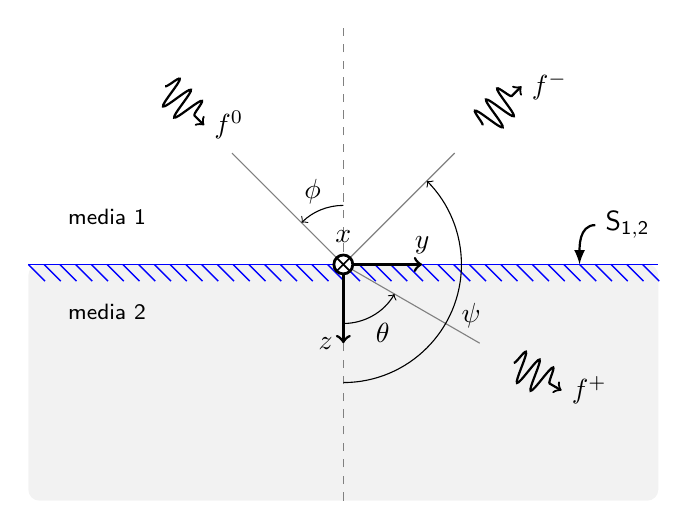
\begin{tikzpicture}[
    media/.style={font={\footnotesize\sffamily}},
    wave/.style={
        decorate,decoration={snake,post length=1.4mm,amplitude=2mm,
        segment length=2mm},thick},
    interface/.style={
        % The border decoration is a path replacing decorator. 
        % For the interface style we want to draw the original path.
        % The postaction option is therefore used to ensure that the
        % border decoration is drawn *after* the original path.
        postaction={draw,decorate,decoration={border,angle=-45,
                    amplitude=0.3cm,segment length=2mm}}},
    ]
    % Round rectangle
    \fill[gray!10,rounded corners] (-4,-3) rectangle (4,0);
    % Interface
    \draw[blue,line width=.5pt,interface](-4,0)--(4,0);
    % Vertical dashed line
    \draw[dashed,gray](0,-3)--(0,3);
    % Coordinates system
    \draw(0,0.15)node[above]{$x$};
    \draw[<->,line width=1pt] (1,0) node[above]{$y$}-|(0,-1) node[left]{$z$};
    % Incidence
    \draw[->,wave]
         (135:3.2cm)--(135:2.5cm)node[right]{$f^0$};
    \draw[gray](0:0cm)--(135:2cm);
    \path (0,0)++(113:1cm)node{$\phi$};
    \draw[->](0,0.75)arc(90:135:.75cm);
    % Transmission
    \draw[->,wave]
         (-30:2.5cm)--(-30:3.2cm)node[right]{$f^+$};
    \draw[gray](0:0cm)--(-30:2cm);
    \path (0,0)++(-60:1cm)node{$\theta$};
    \draw[->] (0,-0.75) arc (-90:-30:.75cm);
    % Reflection
    \draw[->,wave]
         (45:2.5cm)--(45:3.2cm)node[right]{$f^-$};
    \path (0,0)++(-22:1.75cm) node{$\psi$};
    \draw[gray](0:0cm)--(45:2cm);
    \draw[->] (0,-1.5)arc(-90:45:1.5cm);
    % Media names
    \path[media] (-3,.6)  node {media 1}
                 (-3,-.6) node {media 2};

    % $x$ axis
    \filldraw[fill=white,line width=1pt](0,0)circle(.12cm);
    \draw[line width=.6pt] (0,0)
                          +(-135:.12cm) -- +(45:.12cm)
                          +(-45:.12cm) -- +(135:.12cm);
    % Interface pointer
    \draw[-latex,thick](3.2,0.5)node[right]{$\mathsf{S_{1,2}}$}
         to[out=180,in=90] (3,0);
    % To-paths are really useful for drawing curved lines. The above
    % to path is equal to:
    %
    % \draw[-latex,thick](3.2,0.5)node[right]{$\mathsf{S_{1,2}}$}
    %      ..controls +(180:.2cm) and +(up:0.25cm) .. (3,0);
    % Internally the to path is translated to a similar bezier curve,
    % but the to path syntax hides the complexity from the user. 
\end{tikzpicture}
}






\def \tikzexe
{
\begin{circuitikz}%[american voltages]
\draw
  % rotor circuit
  (0,0) to [short, *-] (6,0)
  to [V, l_=$\mathrm{j}{\omega}_m \underline{\psi}^s_R$] (6,2) % rotor emf
  to [R, l_=$R_R$] (6,4) % rotor resistance
  to [short, i_=$\underline{i}^s_R$] (5,4) % rotor current

  % stator circuit
  (0,0) to [open, v^>=$\underline{u}^s_s$] (0,4) % stator voltage
  to [short, *- ,i=$\underline{i}^s_s$] (1,4) % stator current
  to [R, l=$R_s$] (3,4) % stator resistance
  to [L, l=$L_{\sigma}$] (5,4) % leakage inductance
  to [short, i_=$\underline{i}^s_M$] (5,3) % magnetizing current
  to [L, l_=$L_M$] (5,0); % magnetizing inductance
\end{circuitikz}
}

